\documentclass[aspectratio=169]{beamer}

%Textos en español
\usepackage{babel}

% Document metadata
\title{Programs}
\subtitle{iHub-Data, IIIT Hyderabad}
%\author[TL]{Pilot Programs from IIIT Hyderabad}
%\institute{iHub-Data, IIIT Hyderabad}
\date{\today}

% Imagen para la página del título (utilice la opción includegraphics para dimensionarla/ubicarla correctamente)
\titlegraphic{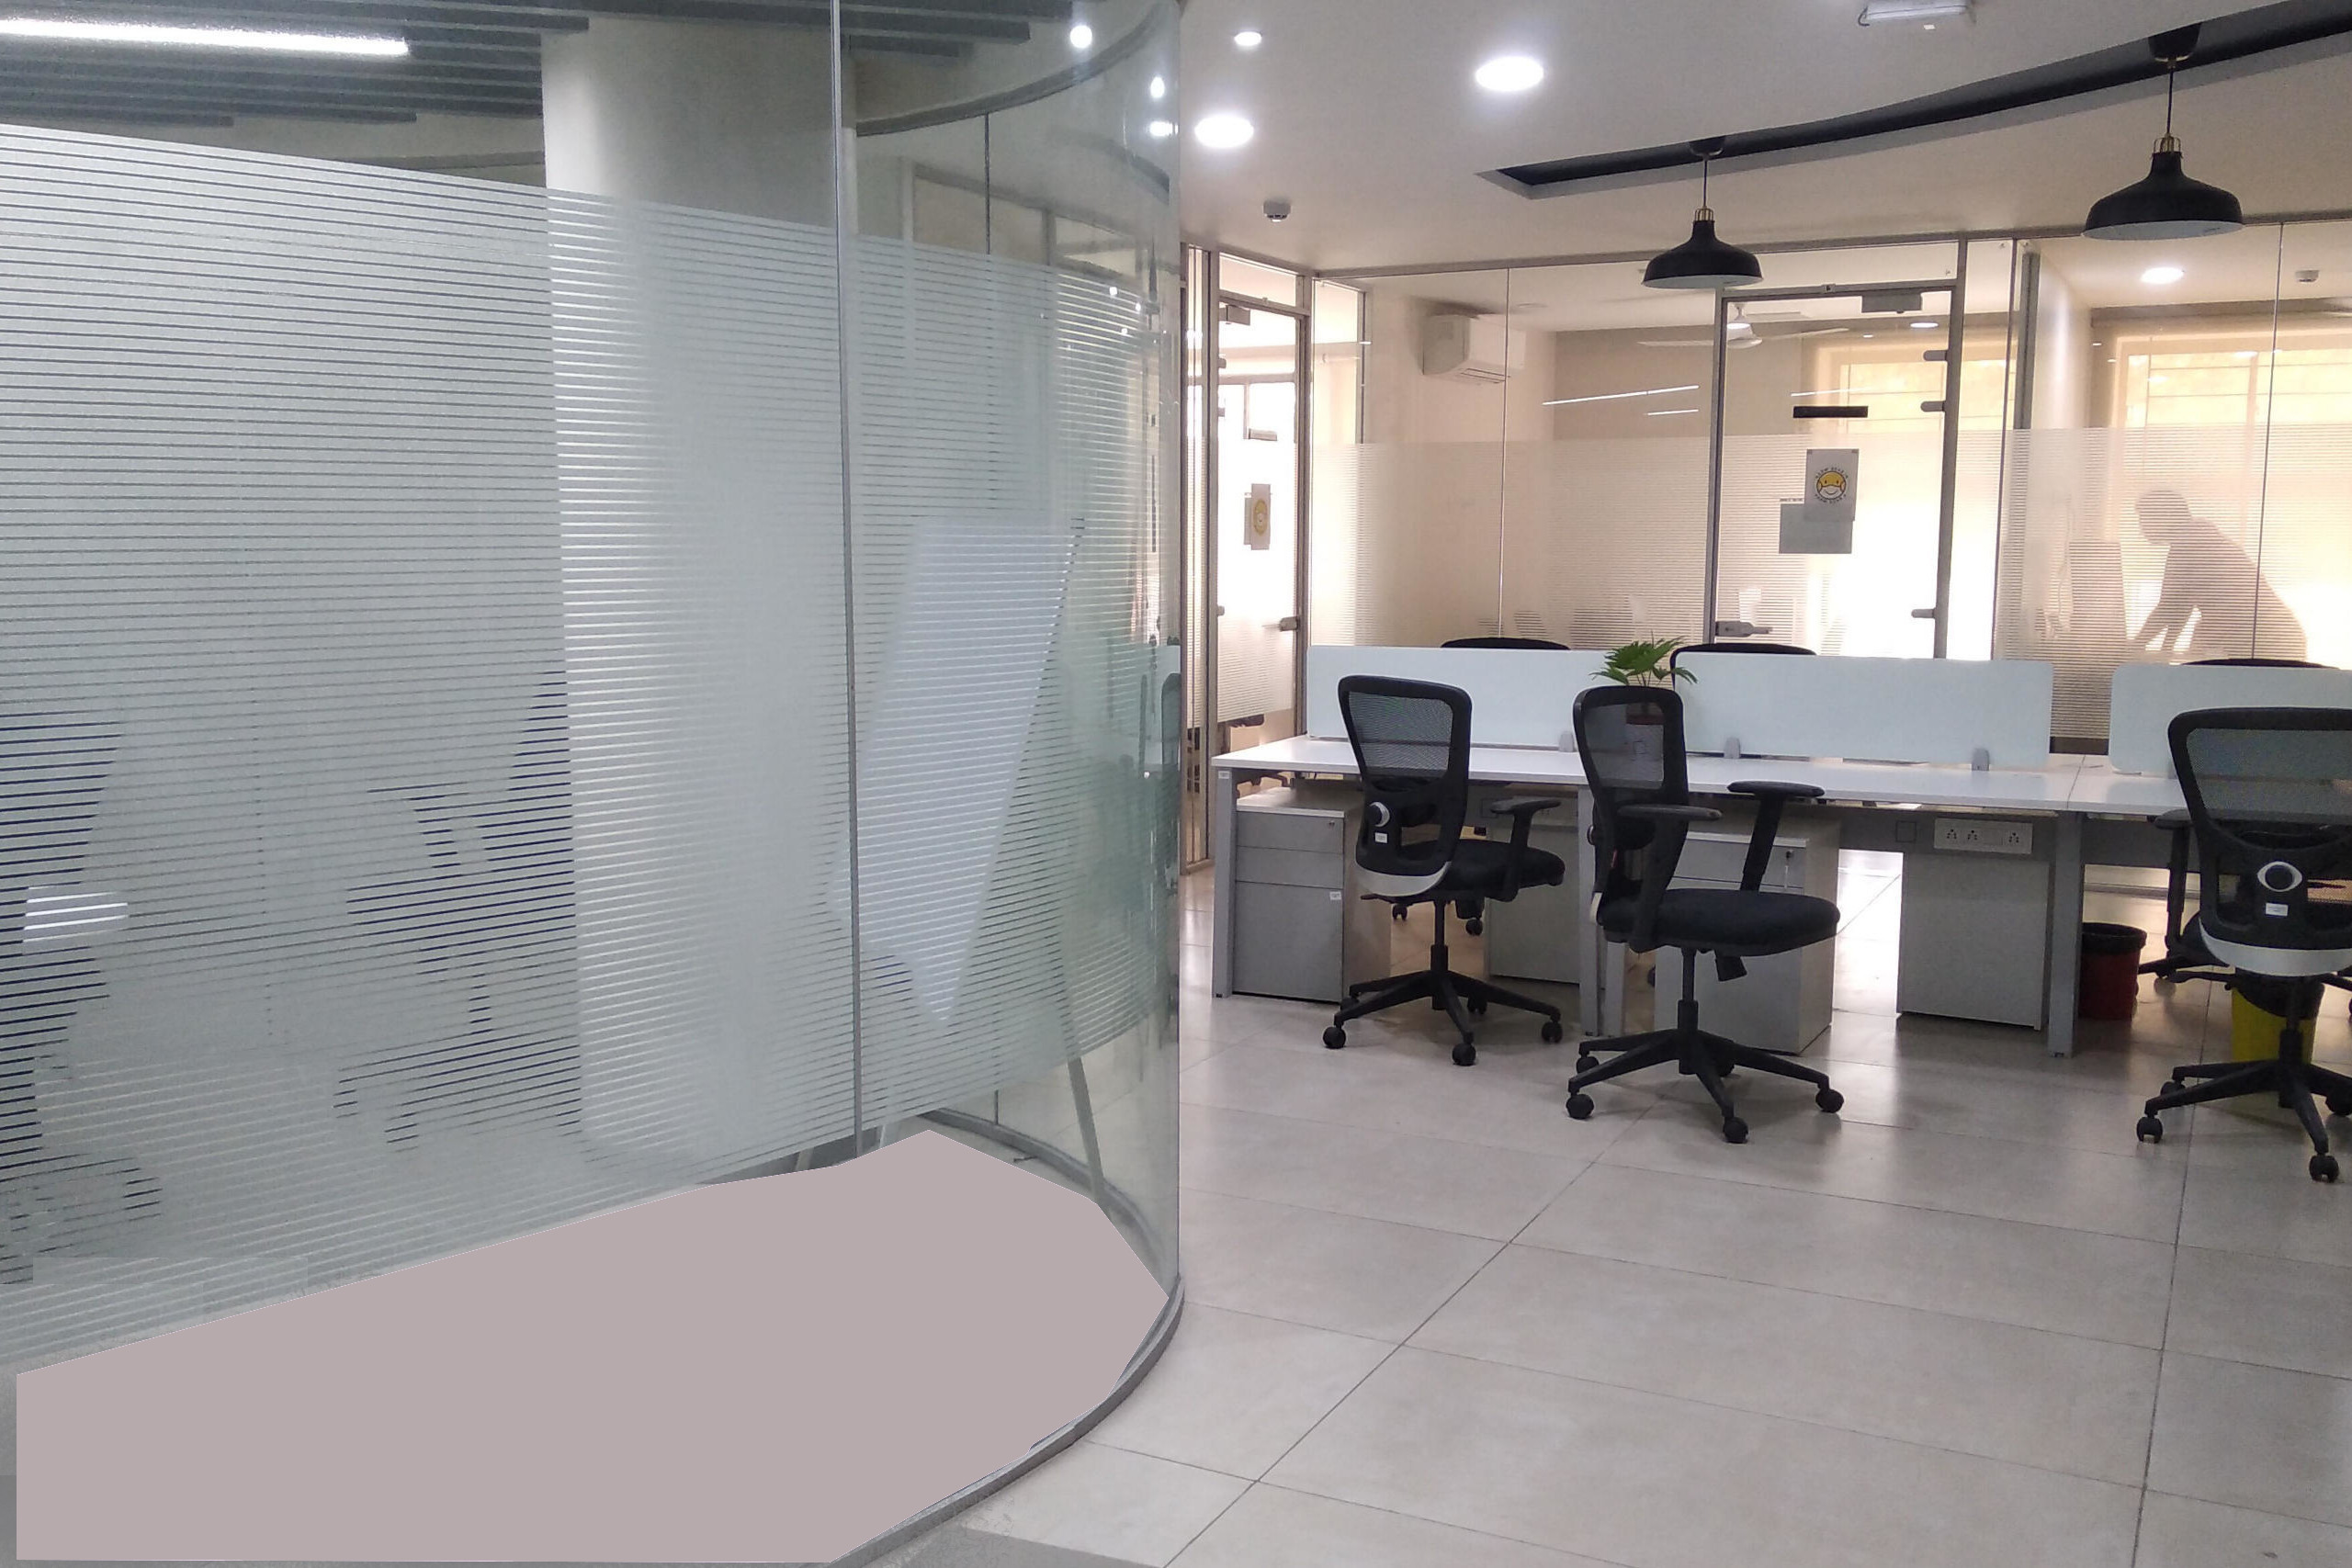
\includegraphics[height=\paperheight]{usach.jpg}}

\usetheme[sectionstyle=style2]{trigon}

% Definir los logotipos a utilizar (comentar si no hay logotipo)
\biglogo{usach_logo.jpg} % Se utiliza sólo en la portada
\smalllogo{logo_small.png} % Se utiliza en la esquina superior derecha de los marcos normales

% ------ Si quieres cambiar los colores por defecto del tema, hazlo aquí ------
\definecolor{tPrim}{HTML}{eA0600}   % 716
\definecolor{tSec}{HTML}{3141B1}    % cool gray
\definecolor{tAccent}{HTML}{502F6C} % 294

 
% ------ Paquetes y definiciones utilizados para esta demostración. Se pueden eliminar ------
\usepackage{appendixnumberbeamer} % To use \appendix command
\pdfstringdefDisableCommands{% Fix hyperref translate warning with \appendix
\def\translate#1{#1}%
}
\usepackage{pgf-pie} % For pie charts 
\usepackage{caption} % For subfigures
\usepackage{subcaption} % For subfigures
\usepackage{xspace}
\newcommand{\themename}{\textbf{\textsc{USACHtheme}}\xspace}
\usepackage[scale=2]{ccicons} % Icons for CC-BY-SA
\usepackage{booktabs} % Better tables


%==============================================================================
%                               COMENZAR DOCUMENTO
%==============================================================================
\begin{document}

%--------------------------------------
% Create title frame
\titleframe

%--------------------------------------
% Table of contents
%\begin{frame}{Overview}
%  \setbeamertemplate{section in toc}[sections numbered]
%  \tableofcontents[hideallsubsections]
%\end{frame}


%==============================================
\section{Programs}
%==============================================
\begin{frame}
  \begin{itemize}
    \item Skill Development
         \begin{enumerate}
        \item 36-week Foundations of Modern Machine Learning (Jan 22 to July 22) 
        \item 50-week Foundations of Modern Machine Learning (Oct 21  to July 22)
        \item 12-week Machine Learning for Chemistry and Drug Design (Mar 22 to Jun 22)
     \end{enumerate}
    \item Outreach Activities
     \begin{enumerate}
        \item MoU with RGUKT institutions
     \end{enumerate}
    \item Fellowships
     \begin {enumerate}
        \item 07 MS and 03 PhD fellowships (Aug 21 to Jul 22)
       \item Mini Symposiums in Dec 21 and Mar 22
     \end{enumerate}
    \item Events
     \begin{enumerate}
       \item International Data Privacy Day 28 Jan 2022
      \item Women in Science and Technology 11 Feb 2022
      \item 10th Workshop on Excitement of Research (245 students) - 21 April 2022
     \end{enumerate}
    \item Visitors
      \begin{enumerate}
         \item Summer Internship Program for (124 students) - May to June 2022
      \end{enumerate}
  \end{itemize}

\end{frame}
%
%%==============================================
%\section{Details}
%%==============================================
%\begin{frame}{\insertsectionhead}
%  \framesubtitle{Programs}
%
%  \begin{itemize}
%    \item Skill Development
%     \begin{enumerate}
%        \item 
%     \end{enumerate}
%    \item Outreach Activities
%    \item Fellowships
%    \item Events
%    \item Visitors
%  \end{itemize}
%
%\end{frame}
%
%
%%==============================================
%\section{50-week Foundations of Modern Machine Learning }
%%==============================================
%
%\subsection{Course Details}
%
%\begin{frame}[fragile=singleslide]{\insertsectionhead}
%  \framesubtitle{\insertsubsectionhead}
%\begin{center}
%\begin{itemize}
%\item Chief Instructors - Prof CV Jawahar, Prof Anoop M, Dr Ravi Kiran 
%\item Sessions handled by large pool of topic experts from IIIT Hyderabad
%\item Live Interactive Session of 1.5hrs duration per week
%\item Distinguished Lectures - once per month
%\item Distributed Personalised Tutorial Sessions - 20 per week
%\item Weekly Mini-projects, Monthly Projects and Quarterly Exams
%\item Enrollment - 250 from all over India
%\item Started in Oct 2021, Expected to end by July 2022
%\end{itemize}
%\end{center}
%\end{frame}
%
%
%%==============================================
%\section{36-week Foundations of Modern Machine Learning }
%%==============================================
%
%\subsection{Course Details}
%
%\begin{frame}[fragile=singleslide]{\insertsectionhead}
%  \framesubtitle{\insertsubsectionhead}
%\begin{center}
%\begin{itemize}
%\item Chief Instructors - Prof CV Jawahar, Prof Anoop M, Dr Ravi Kiran 
%\item Live Interactive Session of 1.5hrs duration per week
%\item Distinguished Lectures - once per month
%\item Distributed Personalised Tutorial Sessions - 20 per week
%\item Weekly Mini-Projects, Monthly Projects and Quarterly Exams
%\item Enrollment - 180 from all over India
%\item Started in Jan 2022, Expected to end by July 2022
%\end{itemize}
%\end{center}
%\end{frame}
%
%
%%==============================================
%\section{8-week Summer Research Internship}
%%==============================================
%
%\subsection{Program Details}
%
%\begin{frame}[fragile=singleslide]{\insertsectionhead}
%  \framesubtitle{\insertsubsectionhead}
%\begin{center}
%\begin{itemize}
%\item Summer Internship Program at IIIT Hyderabad
%\item \textbf{Period : } 16 May onwards for 7/8 weeks
%\item iHub funded Internship Program Rs 10,000 per month
%\item Preliminary Selection from 8000+ students all over India
%\item Two rounds of Screening - MCQs + Essay Writing
%\item 100 students to work in various Research Centres
%\item 90 students listed to work remotely (unpaid)
%\item \textbf{Waiting List : } Another 450 candidates
%\end{itemize}
%\end{center}
%\end{frame}
%
%
%\subsection{Allocation of Interns}
%
%\begin{frame}[fragile=singleslide]{\insertsectionhead}
%  \framesubtitle{\insertsubsectionhead}
%\begin{center}
%\begin{itemize}
%\item All members of faculty  have been alerted to inform details of interns needed
%\item All prospective interns (189 - first list) approached to disclose their preference
%\item iHub will sponsor top 100 performers
%\item Any other support for funding is welcome
%\item Unsupported remote internship is also welcome
%\item Once intern-list is sorted, it will be shared to all faculty - single spreadsheet
%\end{itemize}
%\end{center}
%\end{frame}
%
%
%%==============================================
%\section{10th Edition of Workshop on Excitement of Research}
%%==============================================
%
%\subsection{Program Details}
%
%\begin{frame}[fragile=singleslide]{\insertsectionhead}
%  \framesubtitle{\insertsubsectionhead}
%\begin{center}
%\begin{itemize}
%\item \textbf{Date : } Thursday, 21 April 2022, 9:00am onwards
%\item Invited Audience of over 650 - online Zoom
%\item Prof CV Jawahar : IIIT Hyderabad
%\item Anbumani Subramanian : Principal Research Engineer, Intel Inc
%\item Prof U Deva Priyakumar : IIIT Hyderabad
%\item Prof Syed Azeemuddin : IIIT Hyderabad
%\item CK Raju : iHub-Data
%\end{itemize}
%\end{center}
%\end{frame}
%
%%==============================================
%\section{Future Plans}
%%==============================================
%
%\subsection{Outreach Activities}
%
%\begin{frame}[fragile=singleslide]{\insertsectionhead}
%  \framesubtitle{\insertsubsectionhead}
%\begin{center}
%\begin{itemize}
%\item Scale Online Courses 
%\item Explore Online Internships
%\item Network with Tier-2, Tier-3 technical institutions
%\item Democratise expertise and knowledge
%\end{itemize}
%\end{center}
%\end{frame}
%


%-------------------------------------
%\end{document}
%--------------------------------------


\end{document}
